\documentclass[]{article}
\usepackage{lmodern}
\usepackage{amssymb,amsmath}
\usepackage{ifxetex,ifluatex}
\usepackage{fixltx2e} % provides \textsubscript
\ifnum 0\ifxetex 1\fi\ifluatex 1\fi=0 % if pdftex
  \usepackage[T1]{fontenc}
  \usepackage[utf8]{inputenc}
\else % if luatex or xelatex
  \ifxetex
    \usepackage{mathspec}
  \else
    \usepackage{fontspec}
  \fi
  \defaultfontfeatures{Ligatures=TeX,Scale=MatchLowercase}
\fi
% use upquote if available, for straight quotes in verbatim environments
\IfFileExists{upquote.sty}{\usepackage{upquote}}{}
% use microtype if available
\IfFileExists{microtype.sty}{%
\usepackage{microtype}
\UseMicrotypeSet[protrusion]{basicmath} % disable protrusion for tt fonts
}{}
\usepackage[margin=1in]{geometry}
\usepackage{hyperref}
\hypersetup{unicode=true,
            pdftitle={Assignment2},
            pdfauthor={David Ocepek},
            pdfborder={0 0 0},
            breaklinks=true}
\urlstyle{same}  % don't use monospace font for urls
\usepackage{color}
\usepackage{fancyvrb}
\newcommand{\VerbBar}{|}
\newcommand{\VERB}{\Verb[commandchars=\\\{\}]}
\DefineVerbatimEnvironment{Highlighting}{Verbatim}{commandchars=\\\{\}}
% Add ',fontsize=\small' for more characters per line
\usepackage{framed}
\definecolor{shadecolor}{RGB}{248,248,248}
\newenvironment{Shaded}{\begin{snugshade}}{\end{snugshade}}
\newcommand{\AlertTok}[1]{\textcolor[rgb]{0.94,0.16,0.16}{#1}}
\newcommand{\AnnotationTok}[1]{\textcolor[rgb]{0.56,0.35,0.01}{\textbf{\textit{#1}}}}
\newcommand{\AttributeTok}[1]{\textcolor[rgb]{0.77,0.63,0.00}{#1}}
\newcommand{\BaseNTok}[1]{\textcolor[rgb]{0.00,0.00,0.81}{#1}}
\newcommand{\BuiltInTok}[1]{#1}
\newcommand{\CharTok}[1]{\textcolor[rgb]{0.31,0.60,0.02}{#1}}
\newcommand{\CommentTok}[1]{\textcolor[rgb]{0.56,0.35,0.01}{\textit{#1}}}
\newcommand{\CommentVarTok}[1]{\textcolor[rgb]{0.56,0.35,0.01}{\textbf{\textit{#1}}}}
\newcommand{\ConstantTok}[1]{\textcolor[rgb]{0.00,0.00,0.00}{#1}}
\newcommand{\ControlFlowTok}[1]{\textcolor[rgb]{0.13,0.29,0.53}{\textbf{#1}}}
\newcommand{\DataTypeTok}[1]{\textcolor[rgb]{0.13,0.29,0.53}{#1}}
\newcommand{\DecValTok}[1]{\textcolor[rgb]{0.00,0.00,0.81}{#1}}
\newcommand{\DocumentationTok}[1]{\textcolor[rgb]{0.56,0.35,0.01}{\textbf{\textit{#1}}}}
\newcommand{\ErrorTok}[1]{\textcolor[rgb]{0.64,0.00,0.00}{\textbf{#1}}}
\newcommand{\ExtensionTok}[1]{#1}
\newcommand{\FloatTok}[1]{\textcolor[rgb]{0.00,0.00,0.81}{#1}}
\newcommand{\FunctionTok}[1]{\textcolor[rgb]{0.00,0.00,0.00}{#1}}
\newcommand{\ImportTok}[1]{#1}
\newcommand{\InformationTok}[1]{\textcolor[rgb]{0.56,0.35,0.01}{\textbf{\textit{#1}}}}
\newcommand{\KeywordTok}[1]{\textcolor[rgb]{0.13,0.29,0.53}{\textbf{#1}}}
\newcommand{\NormalTok}[1]{#1}
\newcommand{\OperatorTok}[1]{\textcolor[rgb]{0.81,0.36,0.00}{\textbf{#1}}}
\newcommand{\OtherTok}[1]{\textcolor[rgb]{0.56,0.35,0.01}{#1}}
\newcommand{\PreprocessorTok}[1]{\textcolor[rgb]{0.56,0.35,0.01}{\textit{#1}}}
\newcommand{\RegionMarkerTok}[1]{#1}
\newcommand{\SpecialCharTok}[1]{\textcolor[rgb]{0.00,0.00,0.00}{#1}}
\newcommand{\SpecialStringTok}[1]{\textcolor[rgb]{0.31,0.60,0.02}{#1}}
\newcommand{\StringTok}[1]{\textcolor[rgb]{0.31,0.60,0.02}{#1}}
\newcommand{\VariableTok}[1]{\textcolor[rgb]{0.00,0.00,0.00}{#1}}
\newcommand{\VerbatimStringTok}[1]{\textcolor[rgb]{0.31,0.60,0.02}{#1}}
\newcommand{\WarningTok}[1]{\textcolor[rgb]{0.56,0.35,0.01}{\textbf{\textit{#1}}}}
\usepackage{graphicx,grffile}
\makeatletter
\def\maxwidth{\ifdim\Gin@nat@width>\linewidth\linewidth\else\Gin@nat@width\fi}
\def\maxheight{\ifdim\Gin@nat@height>\textheight\textheight\else\Gin@nat@height\fi}
\makeatother
% Scale images if necessary, so that they will not overflow the page
% margins by default, and it is still possible to overwrite the defaults
% using explicit options in \includegraphics[width, height, ...]{}
\setkeys{Gin}{width=\maxwidth,height=\maxheight,keepaspectratio}
\IfFileExists{parskip.sty}{%
\usepackage{parskip}
}{% else
\setlength{\parindent}{0pt}
\setlength{\parskip}{6pt plus 2pt minus 1pt}
}
\setlength{\emergencystretch}{3em}  % prevent overfull lines
\providecommand{\tightlist}{%
  \setlength{\itemsep}{0pt}\setlength{\parskip}{0pt}}
\setcounter{secnumdepth}{0}
% Redefines (sub)paragraphs to behave more like sections
\ifx\paragraph\undefined\else
\let\oldparagraph\paragraph
\renewcommand{\paragraph}[1]{\oldparagraph{#1}\mbox{}}
\fi
\ifx\subparagraph\undefined\else
\let\oldsubparagraph\subparagraph
\renewcommand{\subparagraph}[1]{\oldsubparagraph{#1}\mbox{}}
\fi

%%% Use protect on footnotes to avoid problems with footnotes in titles
\let\rmarkdownfootnote\footnote%
\def\footnote{\protect\rmarkdownfootnote}

%%% Change title format to be more compact
\usepackage{titling}

% Create subtitle command for use in maketitle
\providecommand{\subtitle}[1]{
  \posttitle{
    \begin{center}\large#1\end{center}
    }
}

\setlength{\droptitle}{-2em}

  \title{Assignment2}
    \pretitle{\vspace{\droptitle}\centering\huge}
  \posttitle{\par}
    \author{David Ocepek}
    \preauthor{\centering\large\emph}
  \postauthor{\par}
      \predate{\centering\large\emph}
  \postdate{\par}
    \date{1/1/2020}


\begin{document}
\maketitle

\begin{Shaded}
\begin{Highlighting}[]
\KeywordTok{library}\NormalTok{(tm)}
\KeywordTok{library}\NormalTok{(wordcloud)}
\KeywordTok{library}\NormalTok{(NLP)}
\KeywordTok{library}\NormalTok{(openNLP)}
\end{Highlighting}
\end{Shaded}

\hypertarget{cleaning}{%
\section{Cleaning}\label{cleaning}}

\begin{center}\rule{0.5\linewidth}{\linethickness}\end{center}

\emph{We read the train data, split the data into y a target label
vector and X a character vector, each entry representing a document.}

\emph{The documents themselves where already transliterated to avoid
character problems and again by R. Because of this there are many string
of the form
\textbackslash\textbackslash\textbackslash\textbackslash x{[}0-9a-fA-F{]}\{2\},
\textbackslash\textbackslash\textbackslash\textbackslash{[}0-9a-fA-F{]},
\textbackslash\textbackslash x{[}0-9a-fA-F{]}\{2\},
\textbackslash\textbackslash{[}0-9a-fA-F{]}, that are not part of the
original text and therefore should be removed.}

\begin{Shaded}
\begin{Highlighting}[]
\NormalTok{train_dir <-}\StringTok{ "C:}\CharTok{\textbackslash{}\textbackslash{}}\StringTok{Users}\CharTok{\textbackslash{}\textbackslash{}}\StringTok{david}\CharTok{\textbackslash{}\textbackslash{}}\StringTok{OneDrive}\CharTok{\textbackslash{}\textbackslash{}}\StringTok{Dokumente}\CharTok{\textbackslash{}\textbackslash{}}\StringTok{GitHub}\CharTok{\textbackslash{}\textbackslash{}}\StringTok{IntelligentSystems}\CharTok{\textbackslash{}\textbackslash{}}\StringTok{insults}\CharTok{\textbackslash{}\textbackslash{}}\StringTok{train.tsv"}
\NormalTok{test_dir <-}\StringTok{ "C:}\CharTok{\textbackslash{}\textbackslash{}}\StringTok{Users}\CharTok{\textbackslash{}\textbackslash{}}\StringTok{david}\CharTok{\textbackslash{}\textbackslash{}}\StringTok{OneDrive}\CharTok{\textbackslash{}\textbackslash{}}\StringTok{Dokumente}\CharTok{\textbackslash{}\textbackslash{}}\StringTok{GitHub}\CharTok{\textbackslash{}\textbackslash{}}\StringTok{IntelligentSystems}\CharTok{\textbackslash{}\textbackslash{}}\StringTok{insults}\CharTok{\textbackslash{}\textbackslash{}}\StringTok{test.tsv"}

\NormalTok{train =}\StringTok{ }\KeywordTok{read.table}\NormalTok{(}\DataTypeTok{file =}\NormalTok{ train_dir, }\DataTypeTok{sep =} \StringTok{'}\CharTok{\textbackslash{}t}\StringTok{'}\NormalTok{, }\DataTypeTok{header =} \OtherTok{TRUE}\NormalTok{, }\DataTypeTok{stringsAsFactors=}\OtherTok{FALSE}\NormalTok{)}
\NormalTok{test =}\StringTok{ }\KeywordTok{read.table}\NormalTok{(}\DataTypeTok{file =}\NormalTok{ test_dir, }\DataTypeTok{sep =} \StringTok{'}\CharTok{\textbackslash{}t}\StringTok{'}\NormalTok{, }\DataTypeTok{header =} \OtherTok{TRUE}\NormalTok{, }\DataTypeTok{stringsAsFactors=}\OtherTok{FALSE}\NormalTok{)}

\NormalTok{handle_special_char <-}\StringTok{ }\ControlFlowTok{function}\NormalTok{(doc)}
\NormalTok{\{}
\NormalTok{  doc =}\StringTok{ }\KeywordTok{iconv}\NormalTok{(doc, }\StringTok{"ASCII"}\NormalTok{, }\StringTok{"ASCII"}\NormalTok{, }\DataTypeTok{sub=}\StringTok{""}\NormalTok{) }\CommentTok{#make sure there are no invalid chars}
                                             \CommentTok{#checked with stri_enc_mark: All are ASCII}
\NormalTok{  doc =}\StringTok{ }\KeywordTok{gsub}\NormalTok{(}\StringTok{"}\CharTok{\textbackslash{}\textbackslash{}\textbackslash{}\textbackslash{}\textbackslash{}\textbackslash{}\textbackslash{}\textbackslash{}}\StringTok{"}\NormalTok{, }\StringTok{"}\CharTok{\textbackslash{}\textbackslash{}\textbackslash{}\textbackslash{}}\StringTok{"}\NormalTok{, doc) }\CommentTok{#remove backslash padding}
\NormalTok{  doc =}\StringTok{ }\KeywordTok{gsub}\NormalTok{(}\StringTok{"}\CharTok{\textbackslash{}\textbackslash{}\textbackslash{}\textbackslash{}}\StringTok{xa0"}\NormalTok{, }\StringTok{" "}\NormalTok{, doc) }\CommentTok{#handle non-carriage return line break}
\NormalTok{  doc =}\StringTok{ }\KeywordTok{gsub}\NormalTok{(}\StringTok{"}\CharTok{\textbackslash{}\textbackslash{}\textbackslash{}\textbackslash{}}\StringTok{xc2"}\NormalTok{, }\StringTok{""}\NormalTok{, doc) }\CommentTok{#handle garbage character}
\NormalTok{  doc =}\StringTok{ }\KeywordTok{gsub}\NormalTok{(}\StringTok{"}\CharTok{\textbackslash{}\textbackslash{}\textbackslash{}\textbackslash{}}\StringTok{x[0-9a-fA-F]\{2\}"}\NormalTok{, }\StringTok{" "}\NormalTok{, doc) }\CommentTok{#handle other UTF-8 characters}
  
\NormalTok{  doc =}\StringTok{ }\KeywordTok{gsub}\NormalTok{(}\StringTok{"}\CharTok{\textbackslash{}\textbackslash{}\textbackslash{}\textbackslash{}\textbackslash{}'}\StringTok{"}\NormalTok{, }\StringTok{"'"}\NormalTok{, doc) }\CommentTok{#handle single parenthesys}
\NormalTok{  doc =}\StringTok{ }\KeywordTok{gsub}\NormalTok{(}\StringTok{"}\CharTok{\textbackslash{}\textbackslash{}\textbackslash{}\textbackslash{}\textbackslash{}"}\StringTok{"}\NormalTok{, }\StringTok{"}\CharTok{\textbackslash{}"}\StringTok{"}\NormalTok{, doc) }\CommentTok{#handle double parenthesys}
\NormalTok{  doc =}\StringTok{ }\KeywordTok{gsub}\NormalTok{(}\StringTok{"}\CharTok{\textbackslash{}\textbackslash{}\textbackslash{}\textbackslash{}}\StringTok{n"}\NormalTok{, }\StringTok{" "}\NormalTok{, doc) }\CommentTok{#handle new line}
\NormalTok{  doc =}\StringTok{ }\KeywordTok{gsub}\NormalTok{(}\StringTok{"}\CharTok{\textbackslash{}\textbackslash{}\textbackslash{}\textbackslash{}}\StringTok{t"}\NormalTok{, }\StringTok{" "}\NormalTok{, doc) }\CommentTok{#handle tab}
\NormalTok{  doc =}\StringTok{ }\KeywordTok{gsub}\NormalTok{(}\StringTok{"}\CharTok{\textbackslash{}\textbackslash{}\textbackslash{}\textbackslash{}}\StringTok{[0-9a-fA-F]"}\NormalTok{, }\StringTok{" "}\NormalTok{, doc) }\CommentTok{#handle other special characters}
  
  \KeywordTok{return}\NormalTok{(doc)}
\NormalTok{\}}

\NormalTok{conn =}\StringTok{ }\KeywordTok{file}\NormalTok{(}\StringTok{"english.stop.txt"}\NormalTok{, }\DataTypeTok{open=}\StringTok{"r"}\NormalTok{)}
\NormalTok{mystopwords =}\StringTok{ }\KeywordTok{readLines}\NormalTok{(conn)}
\KeywordTok{close}\NormalTok{(conn)}

\NormalTok{y =}\StringTok{ }\NormalTok{train[,}\DecValTok{1}\NormalTok{]}
\NormalTok{X =}\StringTok{ }\NormalTok{train[,}\DecValTok{2}\NormalTok{]}
\NormalTok{X <-}\StringTok{ }\KeywordTok{handle_special_char}\NormalTok{(X) }\CommentTok{#Remove special utf8 characters}

\NormalTok{X[}\DecValTok{1}\NormalTok{]}
\end{Highlighting}
\end{Shaded}

\begin{verbatim}
## [1] "Xanax  was  her  death  blow.   That  stuff  is  totally  dangerous  because  you  build  a  tolerance  to  it  so  quickly  and  if  you  stop  abruptly,  you  could  d  ie.   It  is  so  insidious  because  you  keep  taking  it  more  and  more  and  it  affects  your  memory  to  the  point  that  you  forget  how  much  you  took.   You  take  more  because  it  loses  it's  high  effects  yet  its  memory  destroying  effects  get  worse  and  you  get  to  a  point  that  you  don't  even  know  what  you  are  doing  anymore.   Mix  some  serious  partying  in  and  you  have  a  recipe  for  disaster.   She  probably  was  so  drunk  and  drugged  that  she  didn't  know  how  much  Xanax  she  took,  (you  can  easily  forget  that  you  took  a  dose  if  you  have  been  high  on  them  for  days)  went  up  to  her  room,  took  another  big  dose  which  was  the  kil  ler  dose  and  the  rest  is  history. "
\end{verbatim}

\emph{Now that the array of documents is in proper order each document
has to be vectorized. I first anonymize proper nouns with the use of POS
tagging. This has the benefit of injecting the model with knowladge that
all proper nouns should be treated similairly and reducing the
dimensionality of our vector space.}

\emph{To further reduce the vector space, I transform any uppercase
letters to lowercase. Because I have already anonymized the proper
nouns, I can assume there will be a minimal loss in information.}

\emph{Numbers are not neccessary as such they are removed.}

\emph{Common word are removed as they have a low probability of
differentiating between insult and non-insult as there presence in both
on average is almost garranteed.}

\emph{While at a loss to some information I also radicalize the words
therefore allowing the algorithm to find similarity between similair
words.}

\emph{This generates a lot of whitespaces which I minimize to 1
whitespace.}

\begin{Shaded}
\begin{Highlighting}[]
\KeywordTok{detach}\NormalTok{(}\StringTok{"package:ggplot2"}\NormalTok{, }\DataTypeTok{unload=}\OtherTok{TRUE}\NormalTok{)}

\NormalTok{nnp_anonimize <-}\StringTok{ }\ControlFlowTok{function}\NormalTok{(doc)}
\NormalTok{\{}
\NormalTok{sent_ann <-}\StringTok{ }\KeywordTok{Maxent_Sent_Token_Annotator}\NormalTok{()}
\NormalTok{word_ann <-}\StringTok{ }\KeywordTok{Maxent_Word_Token_Annotator}\NormalTok{()}
\NormalTok{pos_ann <-}\StringTok{ }\KeywordTok{Maxent_POS_Tag_Annotator}\NormalTok{()}

\ControlFlowTok{for}\NormalTok{ (i }\ControlFlowTok{in} \DecValTok{1}\OperatorTok{:}\KeywordTok{length}\NormalTok{(doc))}
\NormalTok{\{}
\NormalTok{  s <-}\StringTok{ }\KeywordTok{as.String}\NormalTok{(doc[i])}
  
\NormalTok{  a1 <-}\StringTok{ }\KeywordTok{annotate}\NormalTok{(s, sent_ann)}
\NormalTok{  a2 <-}\StringTok{ }\KeywordTok{annotate}\NormalTok{(s, word_ann, a1)}
\NormalTok{  a2w <-}\StringTok{ }\KeywordTok{subset}\NormalTok{(a2, type }\OperatorTok{==}\StringTok{ "word"}\NormalTok{)}
\NormalTok{  a3 <-}\StringTok{ }\KeywordTok{annotate}\NormalTok{(s, pos_ann, a2)}
\NormalTok{  a3w <-}\StringTok{ }\KeywordTok{subset}\NormalTok{(a3, type }\OperatorTok{==}\StringTok{ "word"}\NormalTok{)}
  
\NormalTok{  tags <-}\StringTok{ }\KeywordTok{vector}\NormalTok{()}
  \ControlFlowTok{for}\NormalTok{ (j }\ControlFlowTok{in} \DecValTok{1}\OperatorTok{:}\KeywordTok{length}\NormalTok{(a3}\OperatorTok{$}\NormalTok{features))}
\NormalTok{    tags <-}\StringTok{ }\KeywordTok{c}\NormalTok{(tags, a3}\OperatorTok{$}\NormalTok{features[[j]]}\OperatorTok{$}\NormalTok{POS)}
  
\NormalTok{  tokenPOS <-}\StringTok{ }\KeywordTok{cbind}\NormalTok{(s[a3w], tags)}
\NormalTok{  nnp_names <-}\StringTok{ }\NormalTok{tokenPOS[tokenPOS[,}\DecValTok{2}\NormalTok{] }\OperatorTok{==}\StringTok{ "NNP"}\NormalTok{, }\DecValTok{1}\NormalTok{] }\CommentTok{#List of proper names}
  
  \ControlFlowTok{if}\NormalTok{ (}\KeywordTok{length}\NormalTok{(nnp_names) }\OperatorTok{==}\StringTok{ }\DecValTok{0}\NormalTok{) }\CommentTok{#no proper nouns here}
    \ControlFlowTok{next}
  
  \ControlFlowTok{for}\NormalTok{ (j }\ControlFlowTok{in} \DecValTok{1}\OperatorTok{:}\KeywordTok{length}\NormalTok{(nnp_names))}
\NormalTok{  \{}
\NormalTok{    doc[i] =}\StringTok{ }\KeywordTok{gsub}\NormalTok{(}\KeywordTok{as.String}\NormalTok{(nnp_names[j]), }\StringTok{"it"}\NormalTok{, doc[i], }\DataTypeTok{fixed=}\OtherTok{TRUE}\NormalTok{)}
\NormalTok{  \}}
\NormalTok{\}}
  
  \KeywordTok{return}\NormalTok{(doc)}
\NormalTok{\}}

\NormalTok{X <-}\StringTok{ }\KeywordTok{nnp_anonimize}\NormalTok{(X)}
\NormalTok{X <-}\StringTok{ }\KeywordTok{Corpus}\NormalTok{(}\KeywordTok{VectorSource}\NormalTok{(X))}
\NormalTok{X <-}\StringTok{ }\KeywordTok{tm_map}\NormalTok{(X, }\KeywordTok{content_transformer}\NormalTok{(tolower)) }\CommentTok{#Transform to lower}
\end{Highlighting}
\end{Shaded}

\begin{verbatim}
## Warning in tm_map.SimpleCorpus(X, content_transformer(tolower)):
## transformation drops documents
\end{verbatim}

\begin{Shaded}
\begin{Highlighting}[]
\NormalTok{X <-}\StringTok{ }\KeywordTok{tm_map}\NormalTok{(X, removePunctuation) }\CommentTok{#Remove punctuations}
\end{Highlighting}
\end{Shaded}

\begin{verbatim}
## Warning in tm_map.SimpleCorpus(X, removePunctuation): transformation drops
## documents
\end{verbatim}

\begin{Shaded}
\begin{Highlighting}[]
\NormalTok{X <-}\StringTok{ }\KeywordTok{tm_map}\NormalTok{(X, removeNumbers) }\CommentTok{#Remove number}
\end{Highlighting}
\end{Shaded}

\begin{verbatim}
## Warning in tm_map.SimpleCorpus(X, removeNumbers): transformation drops
## documents
\end{verbatim}

\begin{Shaded}
\begin{Highlighting}[]
\NormalTok{X <-}\StringTok{ }\KeywordTok{tm_map}\NormalTok{(X, removeWords, }\KeywordTok{stopwords}\NormalTok{(}\StringTok{"english"}\NormalTok{)) }\CommentTok{#Remove stopwords}
\end{Highlighting}
\end{Shaded}

\begin{verbatim}
## Warning in tm_map.SimpleCorpus(X, removeWords, stopwords("english")):
## transformation drops documents
\end{verbatim}

\begin{Shaded}
\begin{Highlighting}[]
\NormalTok{X <-}\StringTok{ }\KeywordTok{tm_map}\NormalTok{(X, removeWords, mystopwords) }\CommentTok{#Remove custom stopwords}
\end{Highlighting}
\end{Shaded}

\begin{verbatim}
## Warning in tm_map.SimpleCorpus(X, removeWords, mystopwords): transformation
## drops documents
\end{verbatim}

\begin{Shaded}
\begin{Highlighting}[]
\NormalTok{X <-}\StringTok{ }\KeywordTok{tm_map}\NormalTok{(X, stemDocument) }\CommentTok{#Get radicals}
\end{Highlighting}
\end{Shaded}

\begin{verbatim}
## Warning in tm_map.SimpleCorpus(X, stemDocument): transformation drops
## documents
\end{verbatim}

\begin{Shaded}
\begin{Highlighting}[]
\NormalTok{X <-}\StringTok{ }\KeywordTok{tm_map}\NormalTok{(X, stripWhitespace) }\CommentTok{#Have only one white space}
\end{Highlighting}
\end{Shaded}

\begin{verbatim}
## Warning in tm_map.SimpleCorpus(X, stripWhitespace): transformation drops
## documents
\end{verbatim}

\begin{Shaded}
\begin{Highlighting}[]
\NormalTok{X[[}\DecValTok{1}\NormalTok{]]}\OperatorTok{$}\NormalTok{content}
\end{Highlighting}
\end{Shaded}

\begin{verbatim}
## [1] "death blow stuff total danger build toler quick stop abrupt insidi take affect memori point forget lose high effect memori destroy effect wors point dont anymor parti recip disast drunk drug didnt easili forget dose high day room big dose kil ler dose rest histori"
\end{verbatim}

\hypertarget{exploration}{%
\section{Exploration}\label{exploration}}

\begin{center}\rule{0.5\linewidth}{\linethickness}\end{center}

\emph{I construct a term document matrix to inspect the frequency of
term occurence and data in general.}

\begin{Shaded}
\begin{Highlighting}[]
\KeywordTok{library}\NormalTok{(ggplot2)}
\end{Highlighting}
\end{Shaded}

\begin{verbatim}
## 
## Attaching package: 'ggplot2'
\end{verbatim}

\begin{verbatim}
## The following object is masked from 'package:NLP':
## 
##     annotate
\end{verbatim}

\begin{Shaded}
\begin{Highlighting}[]
\NormalTok{tdm <-}\StringTok{ }\KeywordTok{TermDocumentMatrix}\NormalTok{(X)}
\NormalTok{tdm}
\end{Highlighting}
\end{Shaded}

\begin{verbatim}
## <<TermDocumentMatrix (terms: 7904, documents: 825)>>
## Non-/sparse entries: 19084/6501716
## Sparsity           : 100%
## Maximal term length: 178
## Weighting          : term frequency (tf)
\end{verbatim}

\begin{Shaded}
\begin{Highlighting}[]
\NormalTok{termFrequency <-}\StringTok{ }\KeywordTok{rowSums}\NormalTok{(}\KeywordTok{as.matrix}\NormalTok{(tdm))}
\KeywordTok{qplot}\NormalTok{(}\KeywordTok{seq}\NormalTok{(}\KeywordTok{length}\NormalTok{(termFrequency)),}\KeywordTok{sort}\NormalTok{(termFrequency), }\DataTypeTok{xlab =} \StringTok{"index"}\NormalTok{, }\DataTypeTok{ylab =} \StringTok{"Freq"}\NormalTok{)}
\end{Highlighting}
\end{Shaded}

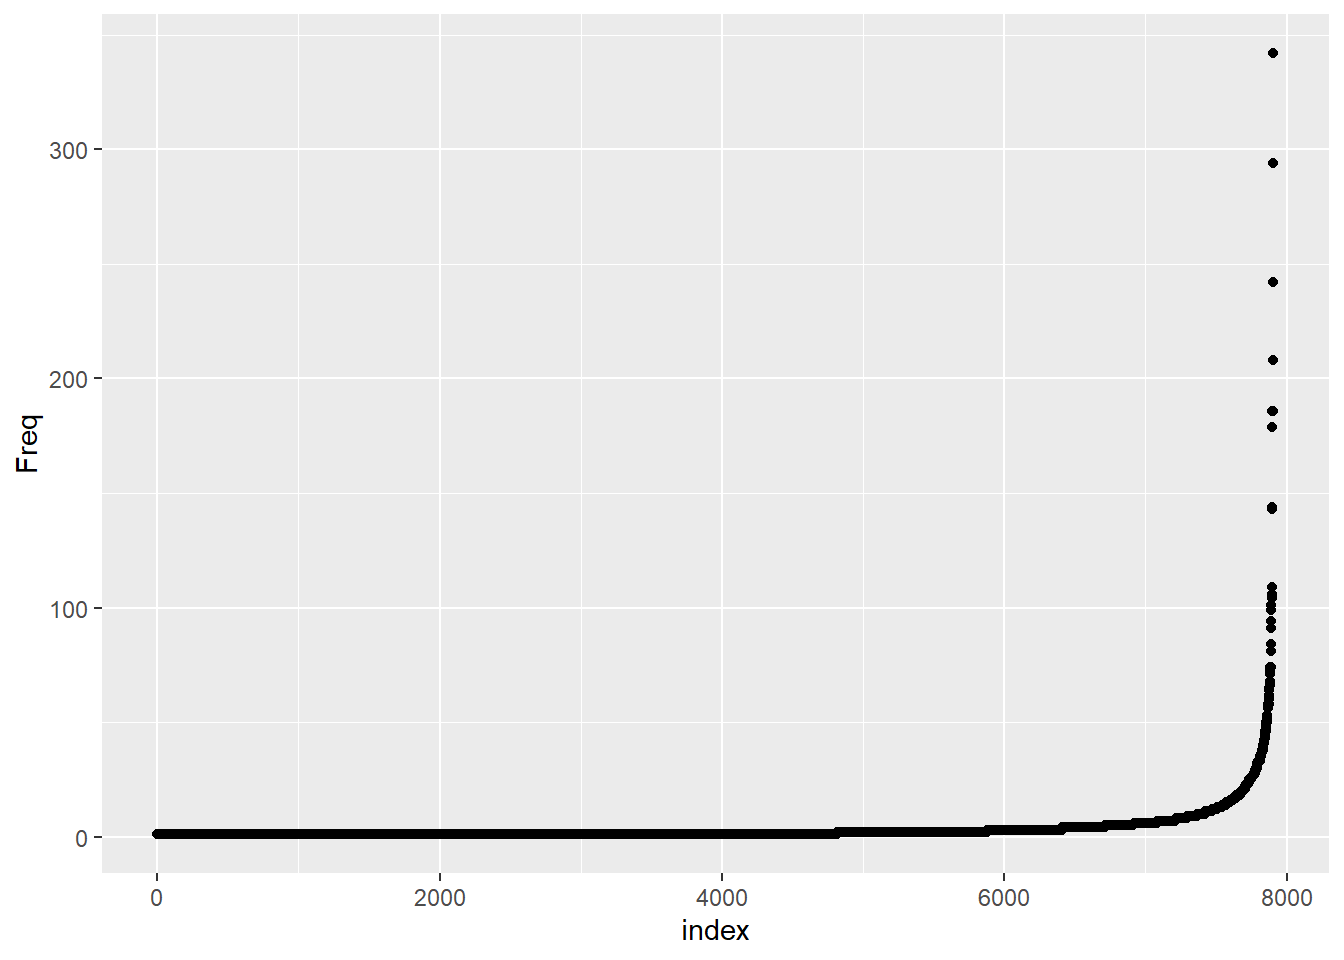
\includegraphics{Assignment2_files/figure-latex/frequency analisys-1.pdf}

\begin{Shaded}
\begin{Highlighting}[]
\KeywordTok{findFreqTerms}\NormalTok{(tdm, }\DataTypeTok{lowfreq=}\DecValTok{100}\NormalTok{)}
\end{Highlighting}
\end{Shaded}

\begin{verbatim}
##  [1] "dont"  "idiot" "thing" "year"  "fuck"  "time"  "good"  "peopl"
##  [9] "make"  "itur"  "yoit"  "yoitr" "itu"
\end{verbatim}

\begin{Shaded}
\begin{Highlighting}[]
\NormalTok{termFrequency <-}\StringTok{ }\KeywordTok{subset}\NormalTok{(termFrequency, termFrequency }\OperatorTok{>=}\StringTok{ }\DecValTok{100}\NormalTok{)}
\KeywordTok{qplot}\NormalTok{(}\KeywordTok{seq}\NormalTok{(}\KeywordTok{length}\NormalTok{(termFrequency)),}\KeywordTok{sort}\NormalTok{(termFrequency), }\DataTypeTok{xlab =} \StringTok{"index"}\NormalTok{, }\DataTypeTok{ylab =} \StringTok{"Freq"}\NormalTok{)}
\end{Highlighting}
\end{Shaded}

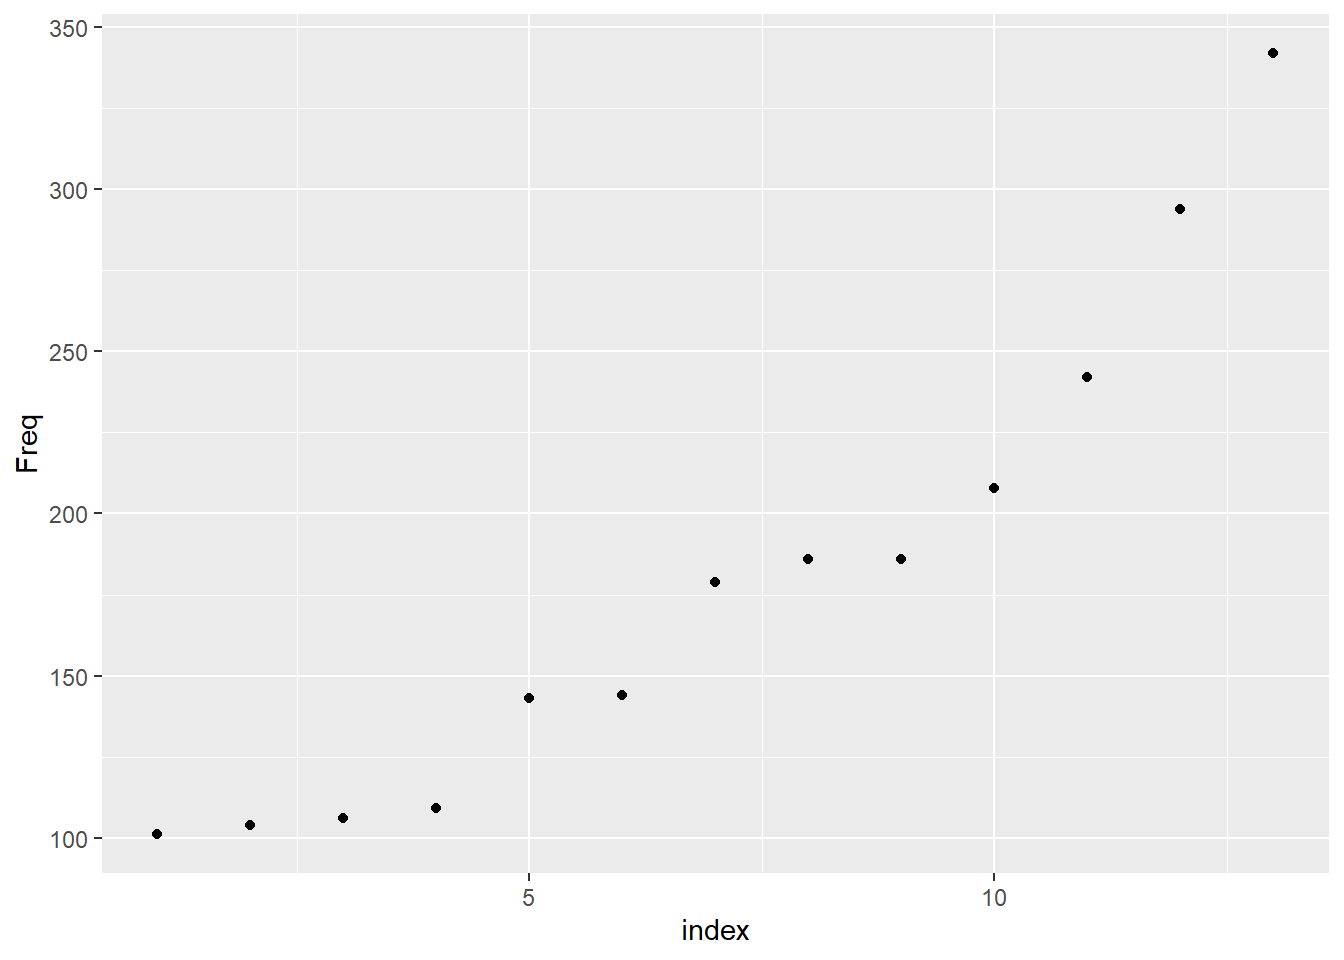
\includegraphics{Assignment2_files/figure-latex/frequency analisys-2.pdf}

\emph{From the graphs it is visible that less than 20 of the almost 8000
terma appear in more than 100 document(the total number of documents is
825). Because of this the term-document and document-term matrix are
100\% sparse. The solution is to reduce the matrix space by balancing
the number of terms in the matrix with the information they present us
with.}

\emph{I perform kmeans clustering projected onto a 2D plane and compare
it to the distribution of the target classes. The results are not great,
but some parts of the distinction between the classes is visible on plot
k=16.}

\begin{Shaded}
\begin{Highlighting}[]
\NormalTok{dtm <-}\StringTok{ }\KeywordTok{DocumentTermMatrix}\NormalTok{(X, }\DataTypeTok{control =} \KeywordTok{list}\NormalTok{(}\DataTypeTok{minDocFreq=}\DecValTok{5}\NormalTok{, }\DataTypeTok{minWordLength=}\DecValTok{4}\NormalTok{, }\DataTypeTok{normalize =} \OtherTok{TRUE}\NormalTok{, }\DataTypeTok{weighting=}\NormalTok{weightTfIdf))}
\end{Highlighting}
\end{Shaded}

\begin{verbatim}
## Warning in weighting(x): empty document(s): 44 109 177 184 239 242 247 307
## 384 437 592 626 700 715 747 773
\end{verbatim}

\begin{Shaded}
\begin{Highlighting}[]
\NormalTok{rowTotals <-}\StringTok{ }\NormalTok{slam}\OperatorTok{::}\KeywordTok{row_sums}\NormalTok{(dtm)}
\NormalTok{dtm <-}\StringTok{ }\NormalTok{dtm[rowTotals }\OperatorTok{>}\StringTok{ }\DecValTok{0}\NormalTok{, ]}
\NormalTok{dtm2 <-}\StringTok{ }\KeywordTok{removeSparseTerms}\NormalTok{(dtm, }\DataTypeTok{sparse=}\FloatTok{0.99}\NormalTok{)}
\NormalTok{mat <-}\StringTok{ }\KeywordTok{as.matrix}\NormalTok{(dtm2)}

\NormalTok{pca <-}\StringTok{ }\KeywordTok{prcomp}\NormalTok{(mat, }\DataTypeTok{scale. =} \OtherTok{TRUE}\NormalTok{, }\DataTypeTok{rank. =} \DecValTok{2}\NormalTok{)}
\NormalTok{comp1 <-}\StringTok{ }\KeywordTok{as.numeric}\NormalTok{(pca}\OperatorTok{$}\NormalTok{x[,}\DecValTok{1}\NormalTok{])}
\NormalTok{comp2 <-}\StringTok{ }\KeywordTok{as.numeric}\NormalTok{(pca}\OperatorTok{$}\NormalTok{x[,}\DecValTok{2}\NormalTok{])}

\NormalTok{kmeansResult <-}\StringTok{ }\KeywordTok{kmeans}\NormalTok{(mat, }\DecValTok{2}\NormalTok{)}
\KeywordTok{qplot}\NormalTok{(comp1, comp2, }\DataTypeTok{color=}\NormalTok{kmeansResult}\OperatorTok{$}\NormalTok{cluster)}
\end{Highlighting}
\end{Shaded}

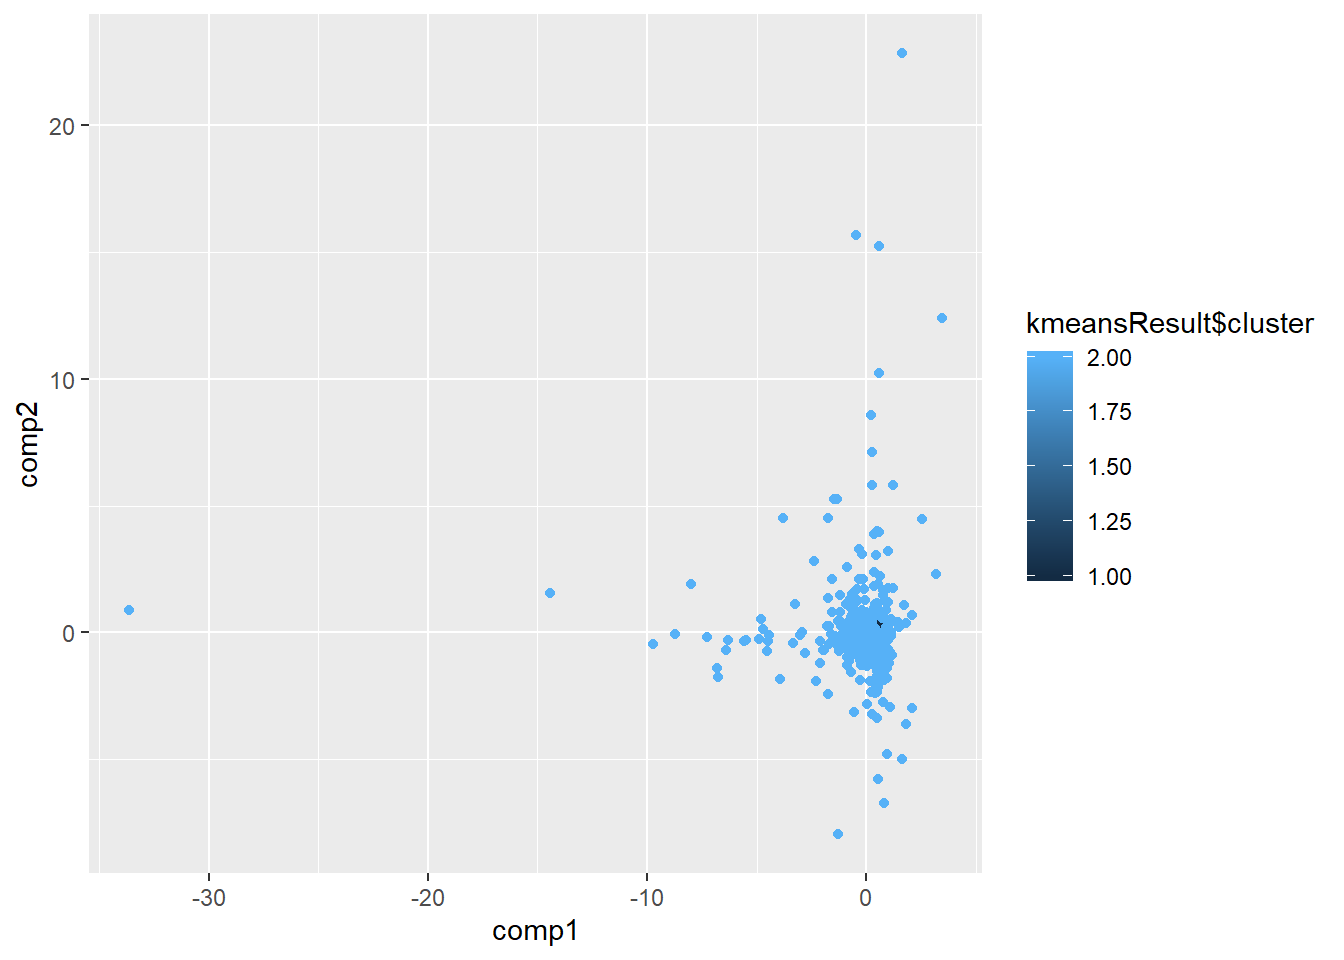
\includegraphics{Assignment2_files/figure-latex/exploration-1.pdf}

\begin{Shaded}
\begin{Highlighting}[]
\NormalTok{kmeansResult <-}\StringTok{ }\KeywordTok{kmeans}\NormalTok{(mat, }\DecValTok{4}\NormalTok{)}
\KeywordTok{qplot}\NormalTok{(comp1, comp2, }\DataTypeTok{color=}\NormalTok{kmeansResult}\OperatorTok{$}\NormalTok{cluster)}
\end{Highlighting}
\end{Shaded}

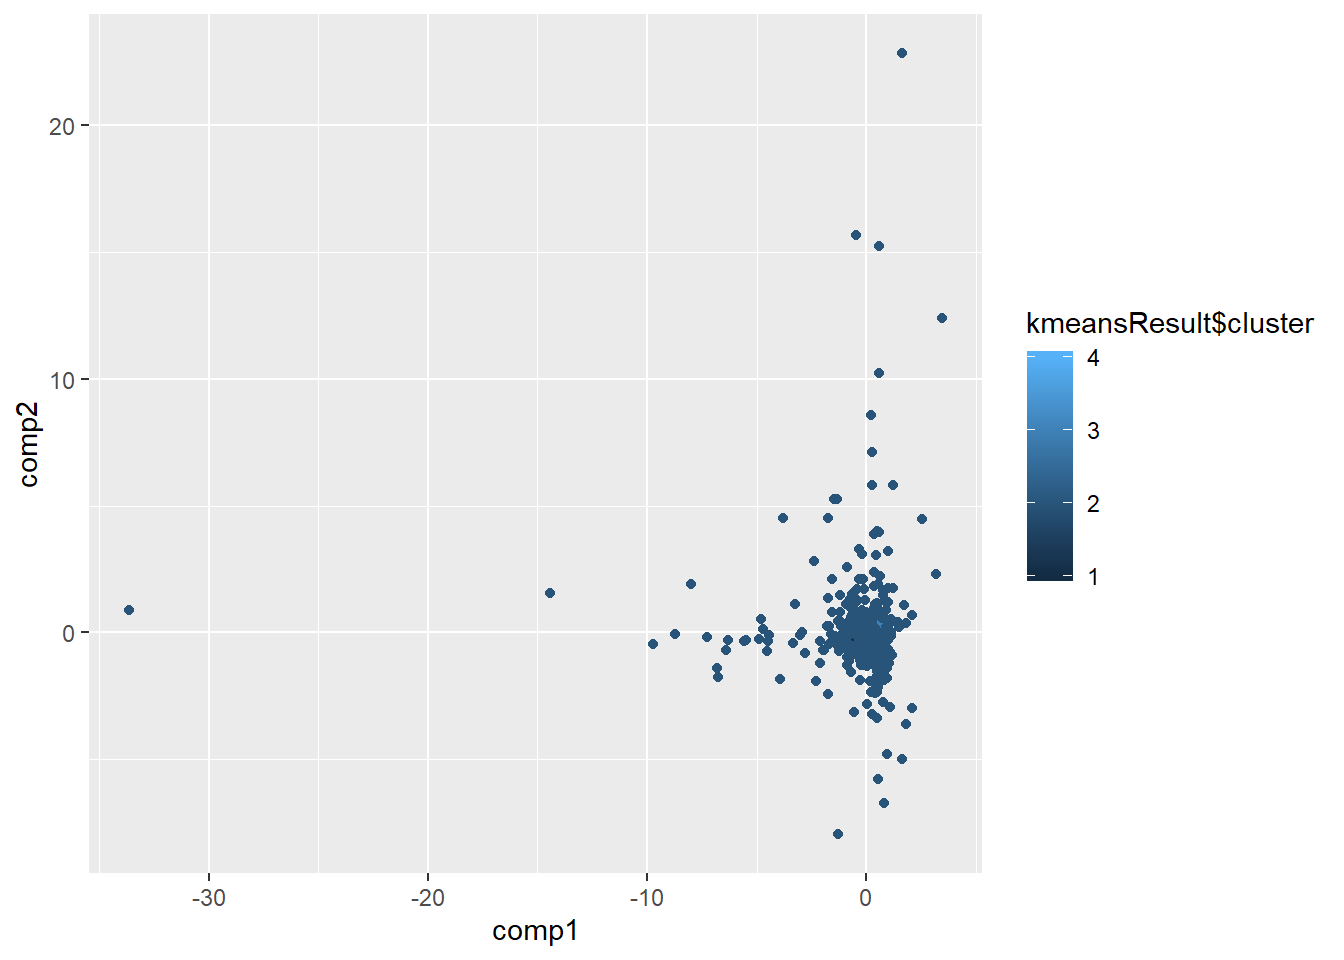
\includegraphics{Assignment2_files/figure-latex/exploration-2.pdf}

\begin{Shaded}
\begin{Highlighting}[]
\NormalTok{kmeansResult <-}\StringTok{ }\KeywordTok{kmeans}\NormalTok{(mat, }\DecValTok{8}\NormalTok{)}
\KeywordTok{qplot}\NormalTok{(comp1, comp2, }\DataTypeTok{color=}\NormalTok{kmeansResult}\OperatorTok{$}\NormalTok{cluster)}
\end{Highlighting}
\end{Shaded}

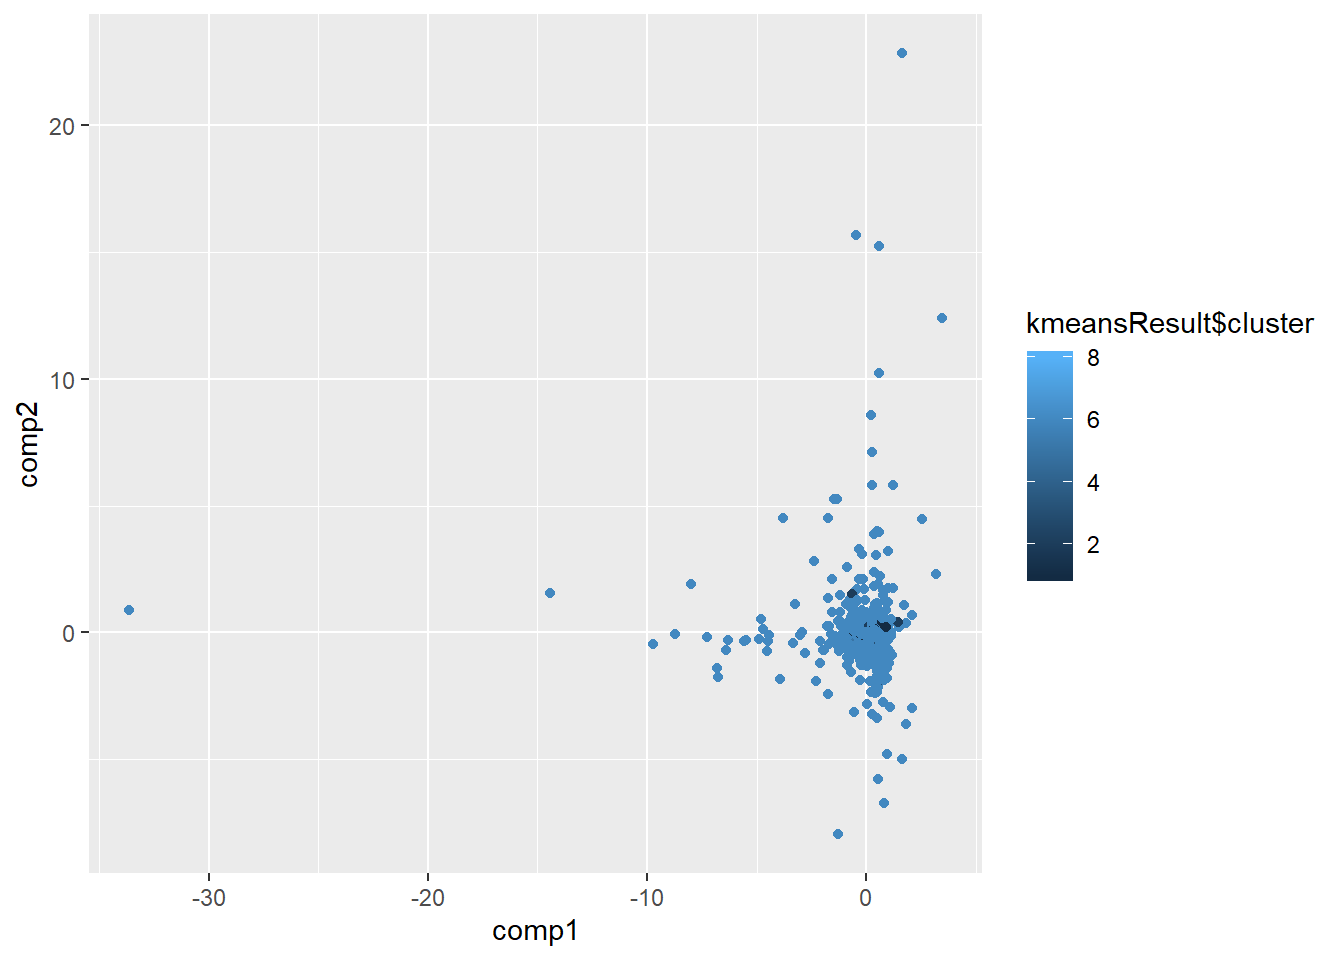
\includegraphics{Assignment2_files/figure-latex/exploration-3.pdf}

\begin{Shaded}
\begin{Highlighting}[]
\NormalTok{kmeansResult <-}\StringTok{ }\KeywordTok{kmeans}\NormalTok{(mat, }\DecValTok{16}\NormalTok{)}
\KeywordTok{qplot}\NormalTok{(comp1, comp2, }\DataTypeTok{color=}\NormalTok{kmeansResult}\OperatorTok{$}\NormalTok{cluster)}
\end{Highlighting}
\end{Shaded}

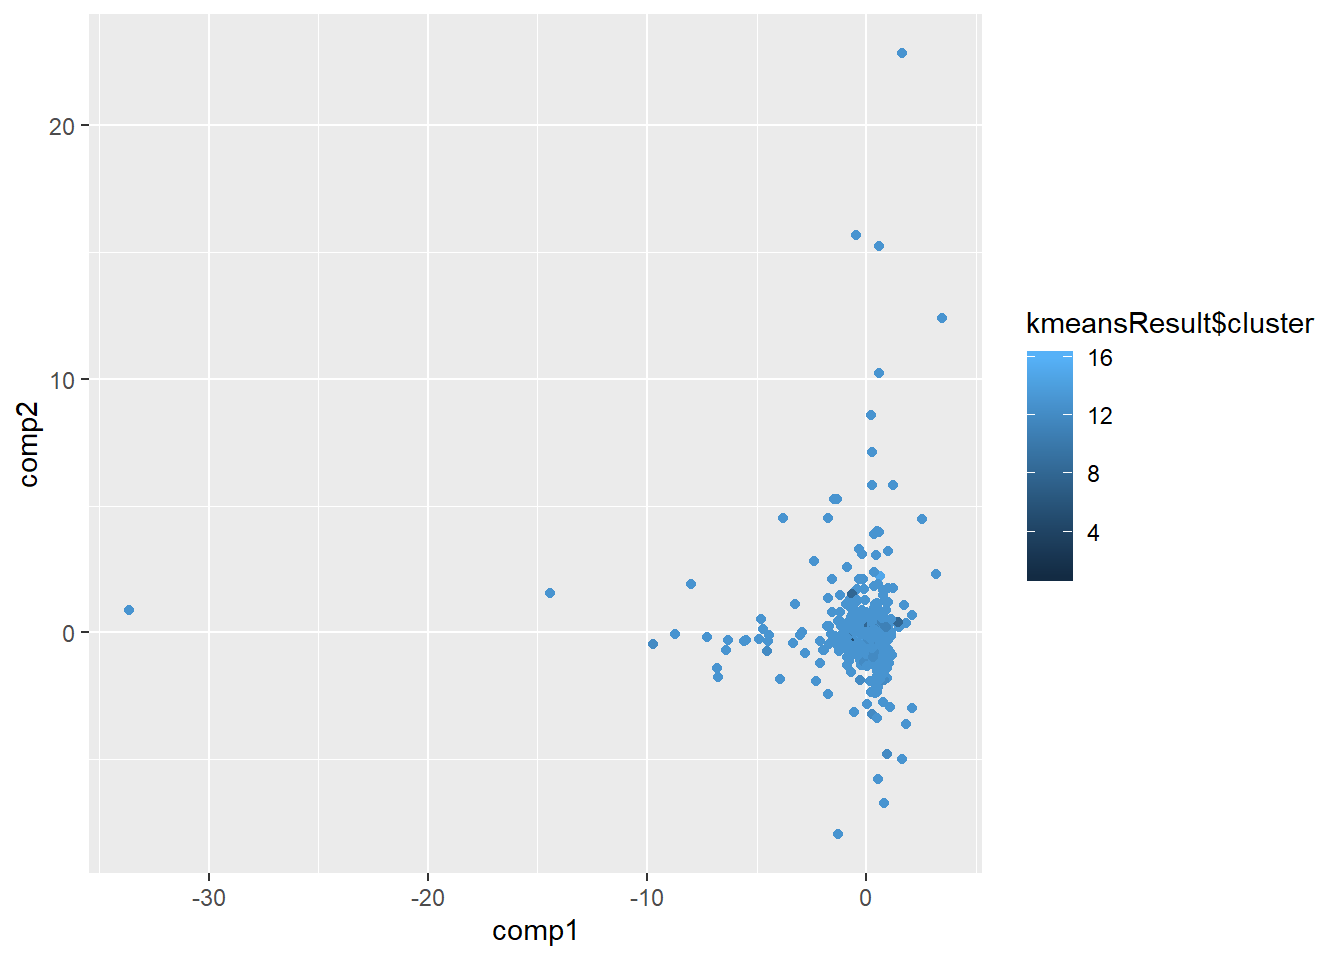
\includegraphics{Assignment2_files/figure-latex/exploration-4.pdf}

\begin{Shaded}
\begin{Highlighting}[]
\KeywordTok{qplot}\NormalTok{(comp1, comp2, }\DataTypeTok{color=}\NormalTok{y[rowTotals }\OperatorTok{>}\StringTok{ }\DecValTok{0}\NormalTok{])}
\end{Highlighting}
\end{Shaded}

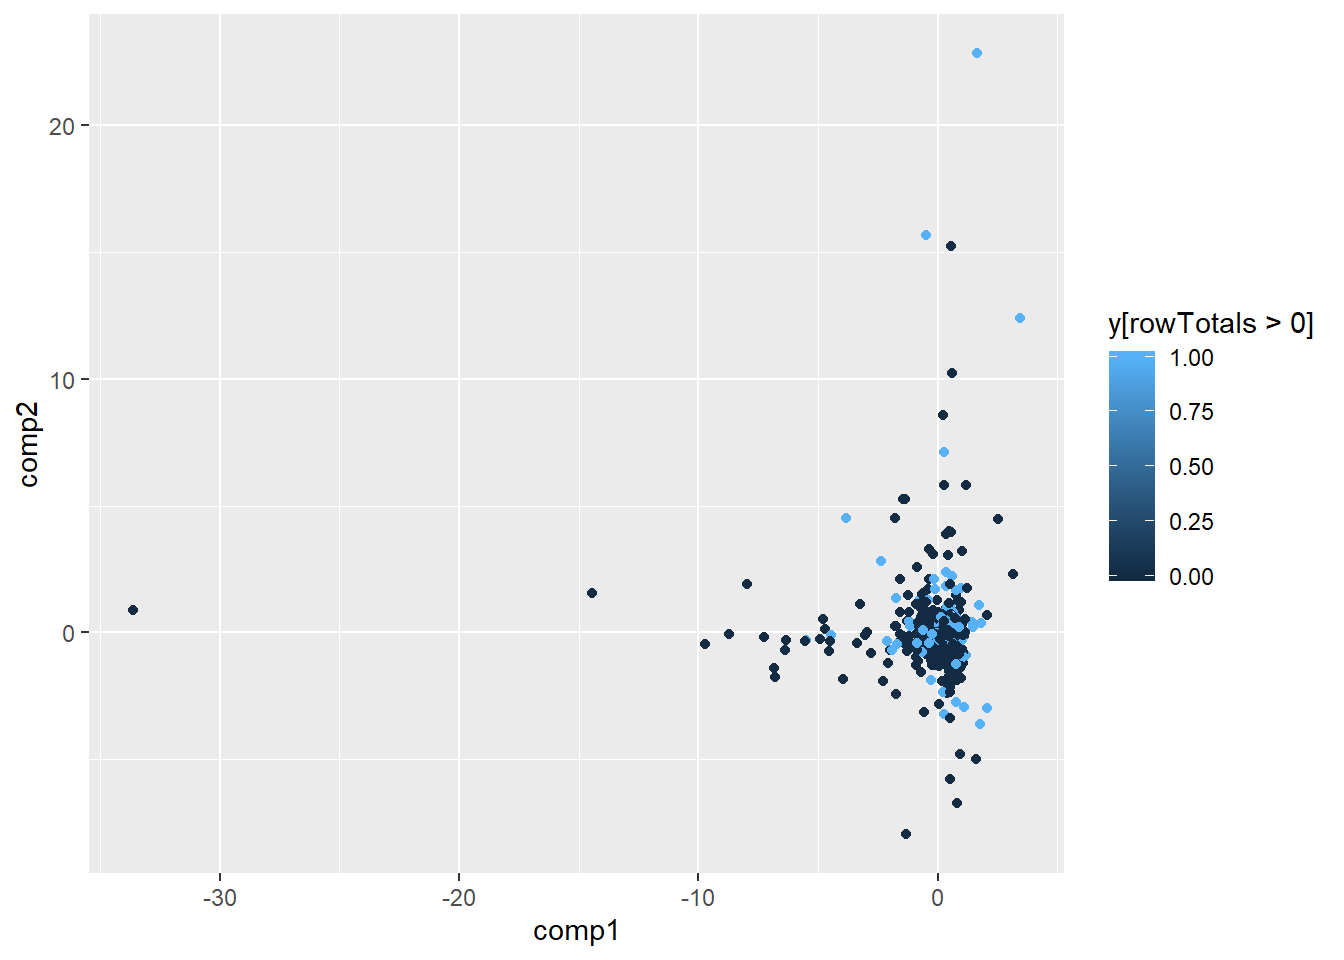
\includegraphics{Assignment2_files/figure-latex/exploration-5.pdf}

\emph{I try a the more robust dbscan clustering with cosine distance.
The resemblance of this plot is much closser to the actual class
distribution. I attribute this to the use of the cosine distance.}

\begin{Shaded}
\begin{Highlighting}[]
\ControlFlowTok{if}\NormalTok{ (}\OperatorTok{!}\KeywordTok{require}\NormalTok{(}\StringTok{"proxy"}\NormalTok{)) }\KeywordTok{install.packages}\NormalTok{(}\StringTok{"proxy"}\NormalTok{)}
\end{Highlighting}
\end{Shaded}

\begin{verbatim}
## Loading required package: proxy
\end{verbatim}

\begin{verbatim}
## Warning: package 'proxy' was built under R version 3.6.2
\end{verbatim}

\begin{verbatim}
## 
## Attaching package: 'proxy'
\end{verbatim}

\begin{verbatim}
## The following objects are masked from 'package:stats':
## 
##     as.dist, dist
\end{verbatim}

\begin{verbatim}
## The following object is masked from 'package:base':
## 
##     as.matrix
\end{verbatim}

\begin{Shaded}
\begin{Highlighting}[]
\ControlFlowTok{if}\NormalTok{ (}\OperatorTok{!}\KeywordTok{require}\NormalTok{(}\StringTok{"dbscan"}\NormalTok{)) }\KeywordTok{install.packages}\NormalTok{(}\StringTok{"dbscan"}\NormalTok{)}
\end{Highlighting}
\end{Shaded}

\begin{verbatim}
## Loading required package: dbscan
\end{verbatim}

\begin{verbatim}
## Warning: package 'dbscan' was built under R version 3.6.2
\end{verbatim}

\begin{Shaded}
\begin{Highlighting}[]
\KeywordTok{library}\NormalTok{(dbscan)}
\KeywordTok{library}\NormalTok{(proxy)}

\NormalTok{dist.matrix =}\StringTok{ }\NormalTok{proxy}\OperatorTok{::}\KeywordTok{dist}\NormalTok{(mat, }\DataTypeTok{method =} \StringTok{"cosine"}\NormalTok{)}
\NormalTok{db_clustering <-}\StringTok{ }\KeywordTok{dbscan}\NormalTok{(dist.matrix, }\DataTypeTok{eps =} \FloatTok{0.7}\NormalTok{, }\DataTypeTok{minPts =} \DecValTok{5}\NormalTok{)}

\KeywordTok{qplot}\NormalTok{(comp1, comp2, }\DataTypeTok{color=}\NormalTok{db_clustering}\OperatorTok{$}\NormalTok{cluster)}
\end{Highlighting}
\end{Shaded}

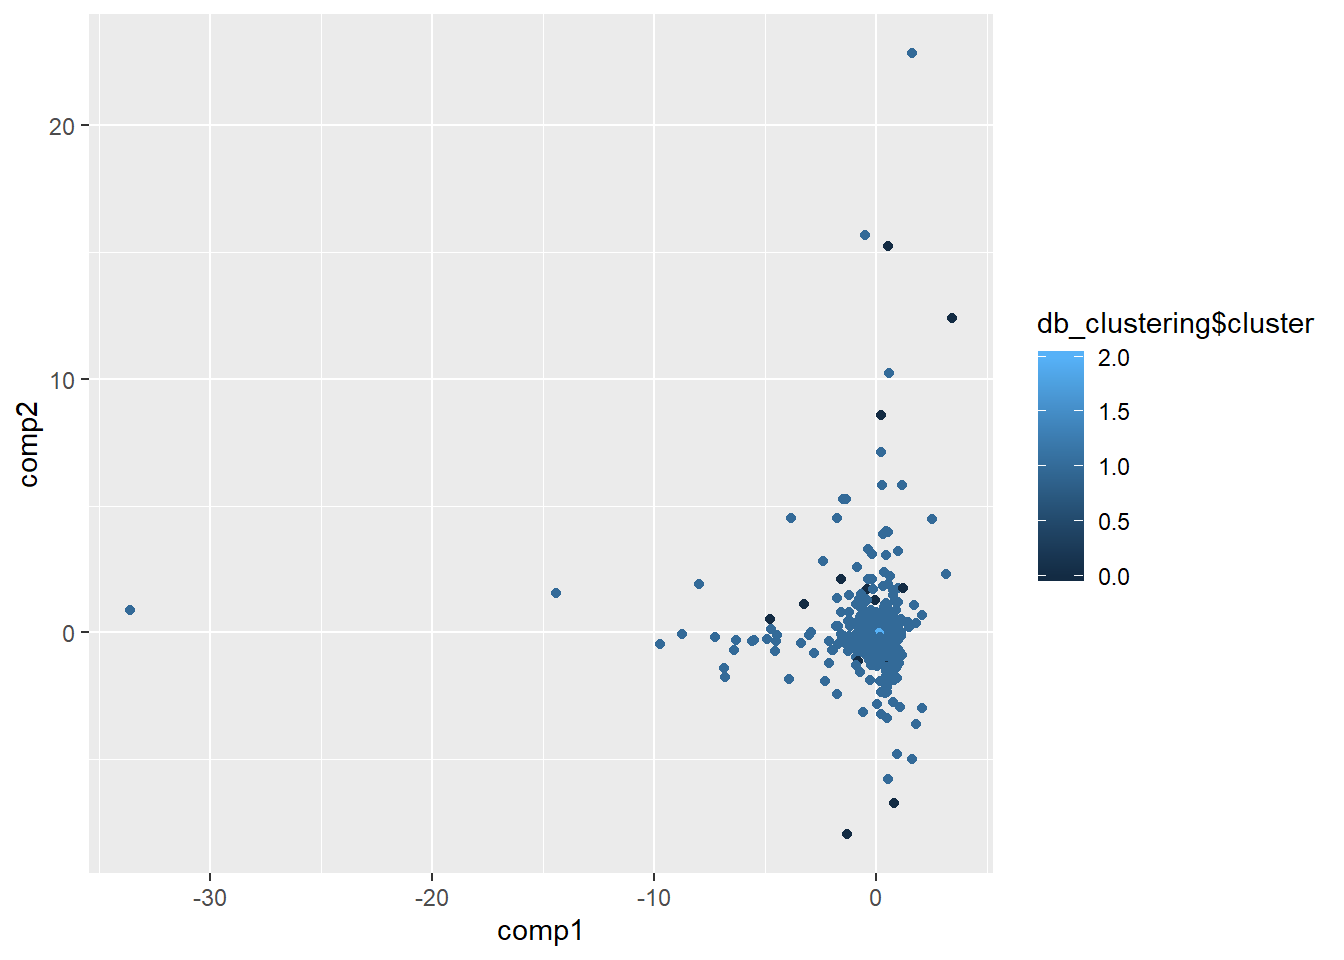
\includegraphics{Assignment2_files/figure-latex/dbscan-1.pdf}

\begin{Shaded}
\begin{Highlighting}[]
\KeywordTok{qplot}\NormalTok{(comp1, comp2, }\DataTypeTok{color=}\NormalTok{y[rowTotals }\OperatorTok{>}\StringTok{ }\DecValTok{0}\NormalTok{])}
\end{Highlighting}
\end{Shaded}

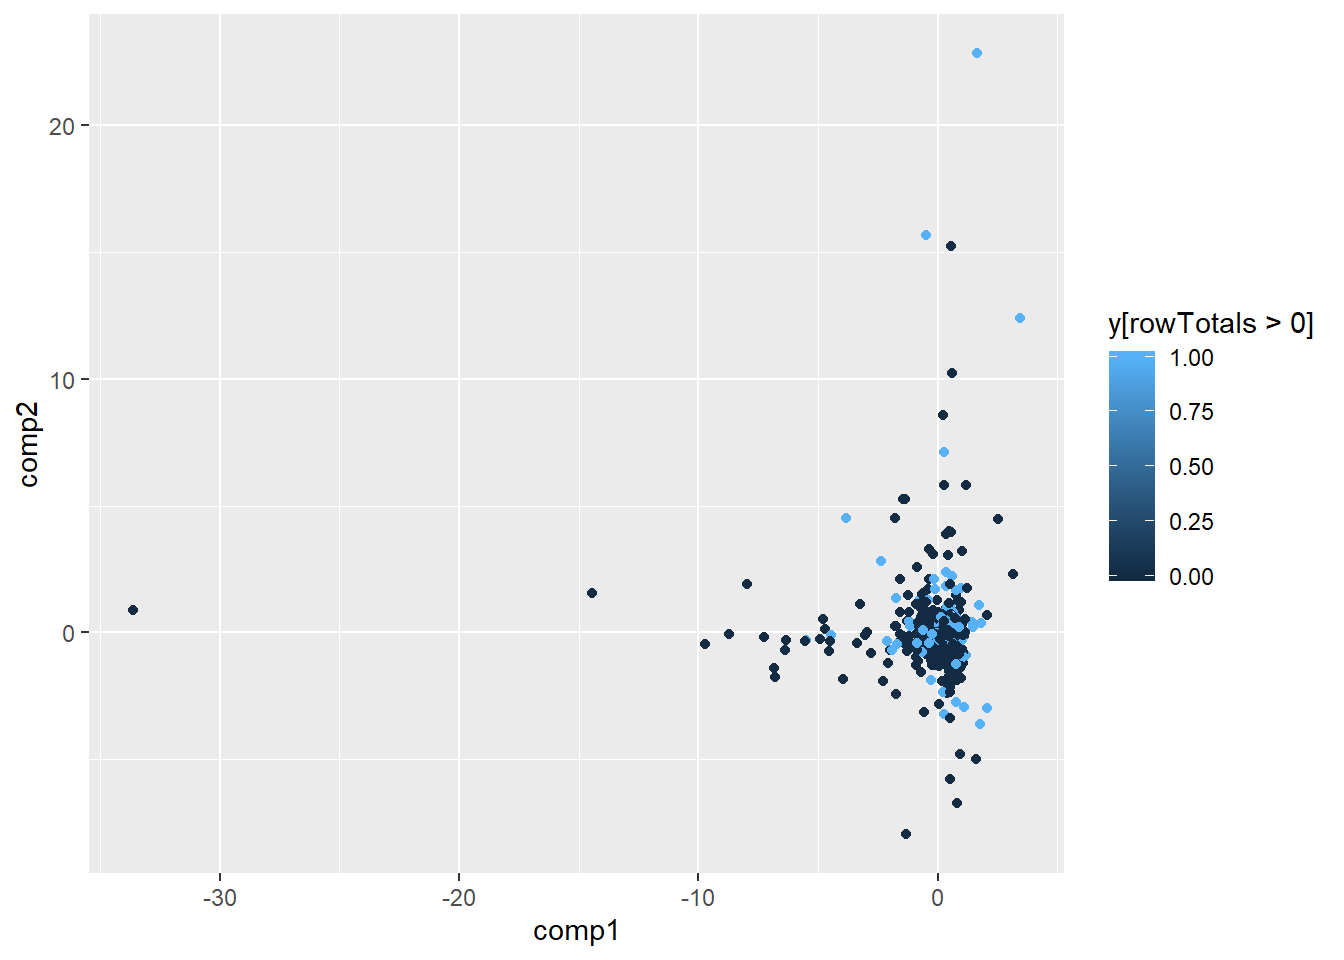
\includegraphics{Assignment2_files/figure-latex/dbscan-2.pdf}

\emph{Dbscan is generraly robust to outlier and the eps and minPoints
were choosen with care meaning the problem is that the vectors
themselves simply don't differ enought. More accuratelly the differences
don't mirror the class distribution enought.}

\emph{I use word2vec to better fit the vector representation to the
class distribution. The fit is visibly better, mainly because it creates
vector representations based on the target classes. Similairy to LDA it
tries to have vectors from the same class be close to each other
i.e.~similair.}

\begin{Shaded}
\begin{Highlighting}[]
\KeywordTok{detach}\NormalTok{(}\StringTok{"package:dbscan"}\NormalTok{, }\DataTypeTok{unload=}\OtherTok{TRUE}\NormalTok{)}
\KeywordTok{detach}\NormalTok{(}\StringTok{"package:proxy"}\NormalTok{, }\DataTypeTok{unload=}\OtherTok{TRUE}\NormalTok{)}

\KeywordTok{library}\NormalTok{(text2vec)}

\NormalTok{X =}\StringTok{ }\NormalTok{train[,}\DecValTok{2}\NormalTok{]}
\NormalTok{X <-}\StringTok{ }\KeywordTok{handle_special_char}\NormalTok{(X)}

\NormalTok{it_train <-}\StringTok{ }\KeywordTok{itoken}\NormalTok{(X, tolower, word_tokenizer)}
\NormalTok{vocab <-}\StringTok{ }\KeywordTok{create_vocabulary}\NormalTok{(it_train)}
\NormalTok{vectorizer <-}\StringTok{ }\KeywordTok{vocab_vectorizer}\NormalTok{(vocab)}
\NormalTok{dtm_train <-}\StringTok{ }\KeywordTok{create_dtm}\NormalTok{(it_train, vectorizer)}
\NormalTok{tfidf <-}\StringTok{ }\NormalTok{TfIdf}\OperatorTok{$}\KeywordTok{new}\NormalTok{()}
\NormalTok{dtm_train_tfidf <-}\StringTok{ }\KeywordTok{fit_transform}\NormalTok{(dtm_train, tfidf)}
\NormalTok{mat <-}\StringTok{ }\KeywordTok{as.matrix}\NormalTok{(dtm_train)}
\NormalTok{kmeansResult <-}\StringTok{ }\KeywordTok{kmeans}\NormalTok{(dtm_train, }\DecValTok{2}\NormalTok{)}
\NormalTok{pca <-}\StringTok{ }\KeywordTok{prcomp}\NormalTok{(mat, }\DataTypeTok{scale. =} \OtherTok{TRUE}\NormalTok{, }\DataTypeTok{rank. =} \DecValTok{2}\NormalTok{)}
\NormalTok{comp1 <-}\StringTok{ }\KeywordTok{as.numeric}\NormalTok{(pca}\OperatorTok{$}\NormalTok{x[,}\DecValTok{1}\NormalTok{])}
\NormalTok{comp2 <-}\StringTok{ }\KeywordTok{as.numeric}\NormalTok{(pca}\OperatorTok{$}\NormalTok{x[,}\DecValTok{2}\NormalTok{])}
\KeywordTok{qplot}\NormalTok{(comp1, comp2, }\DataTypeTok{color=}\NormalTok{kmeansResult}\OperatorTok{$}\NormalTok{cluster)}
\end{Highlighting}
\end{Shaded}

\includegraphics{Assignment2_files/figure-latex/word2vec-1.pdf}

\begin{Shaded}
\begin{Highlighting}[]
\ControlFlowTok{if}\NormalTok{ (}\OperatorTok{!}\KeywordTok{require}\NormalTok{(}\StringTok{"proxy"}\NormalTok{)) }\KeywordTok{install.packages}\NormalTok{(}\StringTok{"proxy"}\NormalTok{)}
\end{Highlighting}
\end{Shaded}

\begin{verbatim}
## Loading required package: proxy
\end{verbatim}

\begin{verbatim}
## Warning: package 'proxy' was built under R version 3.6.2
\end{verbatim}

\begin{verbatim}
## 
## Attaching package: 'proxy'
\end{verbatim}

\begin{verbatim}
## The following objects are masked from 'package:stats':
## 
##     as.dist, dist
\end{verbatim}

\begin{verbatim}
## The following object is masked from 'package:base':
## 
##     as.matrix
\end{verbatim}

\begin{Shaded}
\begin{Highlighting}[]
\ControlFlowTok{if}\NormalTok{ (}\OperatorTok{!}\KeywordTok{require}\NormalTok{(}\StringTok{"dbscan"}\NormalTok{)) }\KeywordTok{install.packages}\NormalTok{(}\StringTok{"dbscan"}\NormalTok{)}
\end{Highlighting}
\end{Shaded}

\begin{verbatim}
## Loading required package: dbscan
\end{verbatim}

\begin{verbatim}
## Warning: package 'dbscan' was built under R version 3.6.2
\end{verbatim}

\begin{Shaded}
\begin{Highlighting}[]
\KeywordTok{library}\NormalTok{(dbscan)}
\KeywordTok{library}\NormalTok{(proxy)}

\NormalTok{dist.matrix =}\StringTok{ }\NormalTok{proxy}\OperatorTok{::}\KeywordTok{dist}\NormalTok{(mat, }\DataTypeTok{method =} \StringTok{"cosine"}\NormalTok{)}
\NormalTok{db_clustering <-}\StringTok{ }\KeywordTok{dbscan}\NormalTok{(dist.matrix, }\DataTypeTok{eps =} \FloatTok{0.7}\NormalTok{, }\DataTypeTok{minPts =} \DecValTok{5}\NormalTok{)}

\KeywordTok{qplot}\NormalTok{(comp1, comp2, }\DataTypeTok{color=}\NormalTok{db_clustering}\OperatorTok{$}\NormalTok{cluster)}
\end{Highlighting}
\end{Shaded}

\includegraphics{Assignment2_files/figure-latex/dbscan for move2vec-1.pdf}

\begin{Shaded}
\begin{Highlighting}[]
\KeywordTok{detach}\NormalTok{(}\StringTok{"package:dbscan"}\NormalTok{, }\DataTypeTok{unload=}\OtherTok{TRUE}\NormalTok{)}
\KeywordTok{detach}\NormalTok{(}\StringTok{"package:proxy"}\NormalTok{, }\DataTypeTok{unload=}\OtherTok{TRUE}\NormalTok{)}
\end{Highlighting}
\end{Shaded}

\begin{Shaded}
\begin{Highlighting}[]
\KeywordTok{qplot}\NormalTok{(comp1, comp2, }\DataTypeTok{color=}\NormalTok{y)}
\end{Highlighting}
\end{Shaded}

\includegraphics{Assignment2_files/figure-latex/class distribution-1.pdf}

\emph{While I used POS tagging earlier when I was anonimizing proper
nouns. It can also be used to inject further knowladge into our data.
(However this raises the dimensionality of are vector space as such it
should be used only with models that have a veriance high enough to
benefit from this.)}

\begin{Shaded}
\begin{Highlighting}[]
\KeywordTok{detach}\NormalTok{(}\StringTok{"package:ggplot2"}\NormalTok{, }\DataTypeTok{unload=}\OtherTok{TRUE}\NormalTok{)}

\NormalTok{X =}\StringTok{ }\NormalTok{train[,}\DecValTok{2}\NormalTok{]}
\NormalTok{X <-}\StringTok{ }\KeywordTok{handle_special_char}\NormalTok{(X) }\CommentTok{#Remove special utf8 characters}

\NormalTok{X[}\DecValTok{1}\NormalTok{]}
\end{Highlighting}
\end{Shaded}

\begin{verbatim}
## [1] "Xanax  was  her  death  blow.   That  stuff  is  totally  dangerous  because  you  build  a  tolerance  to  it  so  quickly  and  if  you  stop  abruptly,  you  could  d  ie.   It  is  so  insidious  because  you  keep  taking  it  more  and  more  and  it  affects  your  memory  to  the  point  that  you  forget  how  much  you  took.   You  take  more  because  it  loses  it's  high  effects  yet  its  memory  destroying  effects  get  worse  and  you  get  to  a  point  that  you  don't  even  know  what  you  are  doing  anymore.   Mix  some  serious  partying  in  and  you  have  a  recipe  for  disaster.   She  probably  was  so  drunk  and  drugged  that  she  didn't  know  how  much  Xanax  she  took,  (you  can  easily  forget  that  you  took  a  dose  if  you  have  been  high  on  them  for  days)  went  up  to  her  room,  took  another  big  dose  which  was  the  kil  ler  dose  and  the  rest  is  history. "
\end{verbatim}

\begin{Shaded}
\begin{Highlighting}[]
\NormalTok{sent_ann <-}\StringTok{ }\KeywordTok{Maxent_Sent_Token_Annotator}\NormalTok{()}
\NormalTok{word_ann <-}\StringTok{ }\KeywordTok{Maxent_Word_Token_Annotator}\NormalTok{()}
\NormalTok{pos_ann <-}\StringTok{ }\KeywordTok{Maxent_POS_Tag_Annotator}\NormalTok{()}

\NormalTok{doctags <-}\StringTok{ }\KeywordTok{vector}\NormalTok{(}\StringTok{"list"}\NormalTok{, }\KeywordTok{length}\NormalTok{(X))}
\NormalTok{docbag <-}\StringTok{ }\KeywordTok{vector}\NormalTok{(}\StringTok{"list"}\NormalTok{, }\KeywordTok{length}\NormalTok{(X))}
\NormalTok{posbag <-}\StringTok{ }\KeywordTok{vector}\NormalTok{(}\StringTok{"list"}\NormalTok{, }\KeywordTok{length}\NormalTok{(X))}

\ControlFlowTok{for}\NormalTok{ (i }\ControlFlowTok{in} \DecValTok{1}\OperatorTok{:}\KeywordTok{length}\NormalTok{(X))}
\NormalTok{\{}
\NormalTok{  s <-}\StringTok{ }\KeywordTok{as.String}\NormalTok{(X[i])}
  
\NormalTok{  a1 <-}\StringTok{ }\KeywordTok{annotate}\NormalTok{(s, sent_ann)}
\NormalTok{  a2 <-}\StringTok{ }\KeywordTok{annotate}\NormalTok{(s, word_ann, a1)}
\NormalTok{  a2w <-}\StringTok{ }\KeywordTok{subset}\NormalTok{(a2, type }\OperatorTok{==}\StringTok{ "word"}\NormalTok{)}
\NormalTok{  a3 <-}\StringTok{ }\KeywordTok{annotate}\NormalTok{(s, pos_ann, a2)}
\NormalTok{  a3w <-}\StringTok{ }\KeywordTok{subset}\NormalTok{(a3, type }\OperatorTok{==}\StringTok{ "word"}\NormalTok{)}
  
\NormalTok{  tags <-}\StringTok{ }\KeywordTok{vector}\NormalTok{()}
  \ControlFlowTok{for}\NormalTok{ (j }\ControlFlowTok{in} \DecValTok{1}\OperatorTok{:}\KeywordTok{length}\NormalTok{(a3}\OperatorTok{$}\NormalTok{features))}
\NormalTok{    tags <-}\StringTok{ }\KeywordTok{c}\NormalTok{(tags, a3}\OperatorTok{$}\NormalTok{features[[j]]}\OperatorTok{$}\NormalTok{POS)}
  
\NormalTok{  tokenPOS <-}\StringTok{ }\KeywordTok{cbind}\NormalTok{(s[a3w], tags)}
\NormalTok{  doctags[[i]] <-}\StringTok{ }\NormalTok{s[a3w]}
\NormalTok{  docbag[[i]] <-}\StringTok{ }\NormalTok{tokenPOS}
\NormalTok{  posbag[[i]] <-}\StringTok{ }\NormalTok{tokenPOS[,}\DecValTok{2}\NormalTok{]}
\NormalTok{\}}

\NormalTok{posbag[[}\DecValTok{1}\NormalTok{]]}
\end{Highlighting}
\end{Shaded}

\begin{verbatim}
##   [1] "NNP"   "VBD"   "PRP$"  "NN"    "NN"    "."     "DT"    "NN"   
##   [9] "VBZ"   "RB"    "JJ"    "IN"    "PRP"   "VBP"   "DT"    "NN"   
##  [17] "TO"    "PRP"   "RB"    "RB"    "CC"    "IN"    "PRP"   "VBP"  
##  [25] "RB"    ","     "PRP"   "MD"    "VB"    "NN"    "."     "PRP"  
##  [33] "VBZ"   "RB"    "JJ"    "IN"    "PRP"   "VBP"   "VBG"   "PRP"  
##  [41] "RBR"   "CC"    "RBR"   "CC"    "PRP"   "VBZ"   "PRP$"  "NN"   
##  [49] "TO"    "DT"    "NN"    "IN"    "PRP"   "VB"    "WRB"   "RB"   
##  [57] "PRP"   "VBD"   "."     "PRP"   "VBP"   "RBR"   "IN"    "PRP"  
##  [65] "VBZ"   "PRP"   "VBZ"   "JJ"    "NNS"   "CC"    "PRP$"  "NN"   
##  [73] "VBG"   "NNS"   "VBP"   "JJR"   "CC"    "PRP"   "VBP"   "TO"   
##  [81] "DT"    "NN"    "IN"    "PRP"   "VBP"   "RB"    "RB"    "VB"   
##  [89] "WP"    "PRP"   "VBP"   "VBG"   "RB"    "."     "NNP"   "DT"   
##  [97] "JJ"    "NN"    "IN"    "CC"    "PRP"   "VBP"   "DT"    "NN"   
## [105] "IN"    "NN"    "."     "PRP"   "RB"    "VBD"   "RB"    "JJ"   
## [113] "CC"    "JJ"    "IN"    "PRP"   "VBD"   "RB"    "VB"    "WRB"  
## [121] "JJ"    "NN"    "PRP"   "VBD"   ","     "NNS"   "MD"    "RB"   
## [129] "VB"    "IN"    "PRP"   "VBD"   "DT"    "NN"    "IN"    "PRP"  
## [137] "VBP"   "VBN"   "JJ"    "IN"    "PRP"   "IN"    "NNS"   "-RRB-"
## [145] "VBD"   "RP"    "TO"    "PRP$"  "NN"    ","     "VBD"   "DT"   
## [153] "JJ"    "NN"    "WDT"   "VBD"   "DT"    "NN"    "NN"    "NN"   
## [161] "CC"    "DT"    "NN"    "VBZ"   "NN"    "."
\end{verbatim}

\hypertarget{modeling}{%
\section{Modeling}\label{modeling}}

\begin{center}\rule{0.5\linewidth}{\linethickness}\end{center}

\emph{The class is biased towards label zero, meaning towards documents
that are not insults or insulting. This is logical because we can assume
that most of online chats are not intended to insult someone.}

\begin{Shaded}
\begin{Highlighting}[]
\NormalTok{tbl <-}\StringTok{ }\KeywordTok{table}\NormalTok{(y)}
\NormalTok{tbl}
\end{Highlighting}
\end{Shaded}

\begin{verbatim}
## y
##   0   1 
## 592 233
\end{verbatim}

\begin{Shaded}
\begin{Highlighting}[]
\NormalTok{tbl[}\DecValTok{2}\NormalTok{]}\OperatorTok{/}\KeywordTok{sum}\NormalTok{(tbl)}
\end{Highlighting}
\end{Shaded}

\begin{verbatim}
##         1 
## 0.2824242
\end{verbatim}


\end{document}
